\documentclass[10pt]{article}
% Эта строка — комментарий, она не будет показана в выходном файле
\usepackage{ucs}
\usepackage[utf8x]{inputenc} % Включаем поддержку UTF8
\usepackage[russian]{babel}  % Включаем пакет для поддержки русского языка
\usepackage{amsmath}
\usepackage{amssymb}
\usepackage{mathtools}

\hoffset=0mm
\voffset=0mm
\textwidth=170mm        % ширина текста
\oddsidemargin=-0mm   % левое поле 25.4 - 5.4 = 20 мм
\textheight=240mm       % высота текста 297 (A4) - 40
\topmargin=-15.4mm      % верхнее поле (10мм)
\headheight=5mm      % место для колонтитула
\headsep=5mm          % отступ после колонтитула
\footskip=8mm         % отступ до нижнего колонтитула

\title{Лабораторная работа № 2.1:
    Определение $C_p/C_v$ по скорости звука в газе    
}
\date{\today}
\author{Зотов Алексей 497}

\begin{document}
        \author {Зотов Алексей 497 гр.}
    \title {Лабораторная работа 2.1 \\  Определение $C_{p}/C_{v}$ по скорости звука в газе}
    \maketitle{}   

    \indent
    \textbf{Цель работы:}
         \begin{enumerate}
         \item Измерение частоты колебаний и длины волны при резонансе звуковых колебаний в газе, заполняющем трубу. 
         \item Определение показателя адиабаты по скорости звука с помощью уравнения состояния идеального газа.
         \end{enumerate}
    \indent
        
        \textbf{В работе используются:} звуковой генератор; электронный осциллограф; теплоизолированная труба; баллон со сжатым углекислым газом; газгольдер. \\ \\


    \textbf{Теория.}

    \textbf{Звуковые волны.} 

    \small{В простых гармонических звуковых волнах, распространяющихся вдоль оси $Ox$, изменение давления $\Delta P$ зависит от координаты $x$ и времени $t$ по закону

    \begin{equation}
        \Delta P(x,t) = P_0 cos(\omega t \pm kx).
    \end{equation}

    Два знака в аргументе косинуса соответствуют двум направлениям распространения волны. Между круговой частотой $\omega$, волновым числом $k$, длиной волны $\lambda$ и скоростью звука $v_\text{зв}$ выполняются соотношения

    \begin{equation}
        v_\text{зв} = \frac{\omega}{k} = \lambda f; \quad k = 2\pi; \quad \omega = 2\pi f;
    \end{equation}
    здесь $f$ — частота волны.
    Важной характеристикой звуковых волн является скорость их
    распространения. Она определяется инерционными и упругими свойствами среды. Скорость распространения продольных волн в безграничной однородной среде определяется выражением:
     
    \begin{equation}
        v_\text{зв} = \sqrt{\frac{dP}{d\rho}}.
    \end{equation}

    Давление $P$ зависит не только от плотности $\rho$, но и от температуры $T$ . Поэтому нужно уточнить, в каком смысле понимается производная $\frac{dP}{d\rho}$.
    Колебания плотности и связанные с ними колебания температуры в звуковой волне происходят настолько быстро, а теплопроводности газов настолько малы, что для таких процессов теплообменом можно пренебречь, так что процесс распространения звука можно считать \textit{адиабатическим}. Следовательно, производную $\frac{dP}{d\rho}$ необходимо рассчитывать для адиабатического процесса.
    }

    \textbf{ Первое начало термодинамики.}

    Из закона сохранения энергии следует, что тепло $Q$, полученное термодинамической системой, расходуется на изменение её внутренней энергии $\Delta U$ и на совершение работы $A$ над внешними телами:
    \begin{equation}
        Q = \Delta U + A
    \end{equation}
    Для бесконечно малого процесса уравнение (4) принимает вид 
    \begin{equation}
        \delta Q = dU + \delta A
    \end{equation}

    Поскольку внутренняя энергия является функцией состояния системы, для её элементарного приращения использован знак полного дифференциала $dU$ , а приращения и тепла, и работы не являются полными дифференциалами, а $Q$ и $A$ — не функции состояния(
    Для интегрирования должен быть задан весь промежуточный процесс, поскольку результат будет зависеть от его вида, а не только от начального и конечного состояний).

    \textbf{ Работа газа.}

    Рассмотрим расширение газа в цилиндре, закрытом подвижным поршнем. На поршень действует сила $F$ , равная произведению давления газа $F$ на площадь поршня $S$. При смещении на малую величину $dx$ газ совершает работу
    \begin{equation}
        \delta A = F dx = P S dx = P dV.
    \end{equation}
    где $dV$  — малое изменение объёма газа.
    Значит полная работа при некотором процессе имеет вид:
    \begin{equation}
        A = \int P(V) dV
    \end{equation}
    А первое начало термодинамики для газов после использования формулы (6) будет иметь вид:
    \begin{equation}
        \delta Q = dU + P dV
    \end{equation}

    \textbf{Теплоемкость}
    Отношение количества тепла $\delta Q$, поглощённого $\nu$ молями газа при некотором процессе, который обозначим индексом $x$, к повышению его температуры на $dT$, делённое на число молей $\nu$, называется \textit{молярной теплоемкостью газа}:

    \begin{equation}
        C = \bigg(\frac{\delta Q}{dT}\bigg)_x / \nu
    \end{equation}

    Будем считать что $U = U(V,T)$ (так как система описывается тремя параметрами: $V,T,P$ но при этом есть уравнение Менделеева-Клапейрона: $P = P(V,T)$).
    Значит полный дифференциал для $U$ имеет следующий вид:

    \begin{equation}
        dU = \bigg(\frac{\delta U}{\delta T}\bigg)_V dT + \bigg(\frac{\delta U}{\delta V}\bigg)_T dV
    \end{equation}

    Подставим его в первое начало термодинамики:

    $  \delta Q = dU + \delta A =  \bigg(\frac{\delta U}{\delta T}\bigg)_V dT + \bigg(\frac{\delta U}{\delta V}\bigg)_T dV + PdV = \bigg(\frac{\delta U}{\delta T}\bigg)_V dT + \bigg[P + \bigg(\frac{\delta U}{\delta V}\bigg)_T \bigg] dV $

    Разделив все на $dT$ найдем теплоемкость $C_x$ в процессе x:

    \begin{equation}
        C_x = C_v + \bigg[P + \bigg(\frac{\delta U}{\delta V}\bigg)_T \bigg] \bigg(\frac{\delta V}{\delta T}\bigg)_x
    \end{equation}

    Здесь производная $\bigg(\frac{\delta V}{\delta T}\bigg)_x$ вычисляется с учётом процесса $x$, при котором происходит подвод тепла, например, при постоянном объеме $(x = V)$, при постоянном давлении $(x = P)$ или другом условии. Величина $C_v = \bigg(\frac{\delta U}{\delta T}\bigg)_V$ в формуле (11) является теплоемкостью при постоянном объqме (Действительно, это определение совпадает с определением теплоемкости, так как в процессе $V = const$ выполняется $\delta A = 0$ а значит $\delta U = dQ$).

    \textbf{Теплоёмкость идеального газа.}
    В модели идеального газа внутренняя энергия определяется только кинетической энергией движения молекул, следовательно, внутренняя энергия идеального газа не зависит от объема: $\bigg(\frac{\delta U}{\delta V}\bigg)_T = 0$.

    Тогда формула (11) станет более простой:

    \begin{equation}
        C_x = C_v + P \bigg(\frac{\delta V}{\delta T}\bigg)_x
    \end{equation}

    Используя уравнение Менделеева-Клапейрона ($PV = \nu RT$),
    для $C_p$ (то есть процесса $x = P$ с постоянным давлением) получим:

    \begin{equation}
        C_p - C_v = R
    \end{equation}
    где $C_p, C_v$ - \textit{молярные} теплоемкости при постоянных давлении и объеме соответсвенно.

    Отношение этих теплоемкостей называется показателем адиабаты:

    \begin{equation}
        \gamma = \frac{C_p}{C_v}
    \end{equation}

    В нешироком диапазоне температур $C_v$ можно считать постоянной, что соответствует пропорциональности внутренней энергии газа его температуре:

    \begin{equation}
        U = \nu \int C_v dT = \nu C_v T
    \end{equation}

    Энергия, переданная молекуле, распределяется между различными формами её движения: поступательным, вращательным и колебательным. В статистической физике доказывается теорема о равномерном распределении энергии между степенями свободы молекулы, согласно которой на каждую степень свободы приходится в среднем энергия, равная $\frac{RT}{2 N_A}$

    При $i$ степенях свободы, внутренняя энергия $U$ одного моля такого газа и величина $C_v$ равны соответственно

    \begin{equation}
        U = \frac{i}{2}RT; \quad C_v = \frac{iR}{2}; 
    \end{equation}

    где $R = 8,31 \text{Дж}/\text{(моль · К)}$ — универсальная газовая постоянная, $N_A = 6,02 · 1023 \text{моль}^{−1}$ — количество молекул в моле вещества (число Авогадро).
    В рассматриваемом приближении для показателя адиабаты в соответствии с (13) и (14) получим

    \begin{equation}
        \gamma = \frac{i+2}{i}
    \end{equation}

    \textbf{Адиабатический процесс.}

    Квазистатический процесс, происходящий без теплообмена с окружающей средой, называется адиабатическим.
    Из первого начала термодинамики (6) при $\delta Q = 0$ для $\nu$ молей идеального газа, у которого $dU = \nu C_v dT$, получим:

    \begin{equation}
        \nu C_v dt + P dV = 0,
    \end{equation}

    А так как $PV = \nu RT$, получаем: 

    \begin{equation}
        C_v \frac{dT}{T} + R \frac{dV}{V} = 0
    \end{equation}

    Далее интегрируя и вновь используя уравнение состояния, получим:

    \begin{equation}
        PV^{\gamma} = const
    \end{equation}

    (адиабата Пуассона)

    \textbf{Скорость звука}
    Распространение звуковой волны в газе происходит адиабатически. Сжатия и разрежения в газе сменяют друг друга настолько быстро, что теплообмен между слоями газа, имеющими разные температуры, не успевает произойти. Используя полученное уравнение адиабаты идеального газа, найдем скорость звука по общей формуле (3).

    Заменим в уравнении Пуассона $PV^{\gamma} = const$ объем на плотность $\rho = \frac{m}{V}$ , после чего получим $P = const \rho^{\gamma} $. Тогда после логарифмирования и дифференцирования этого выражения имеем:

    \begin{equation}
        \frac{dP}{P} = \gamma \frac {d\rho}{\rho}, \quad \text{или} \quad \bigg(\frac{dP}{d\rho}\bigg)_\text{адиаб} = \gamma \frac{P}{\rho},
    \end{equation}

    тогда для скорости звука получаем:

    \begin{equation}
        v_\text{зв}^2 = \bigg(\frac{dP}{d\rho}\bigg)_\text{адиаб} = \gamma \frac{P}{\rho} = \gamma \frac{RT}{\mu},
    \end{equation}
    где $\mu$ - молярная масса газа.

    Преобразуя, получим:

    \begin{equation}
        \gamma = \frac{\mu}{RT}v_\text{зв}^2
    \end{equation}

    Таким образом, для определения показателя адиабаты достаточно измерить температуру газа и скорость распространения звука (молярная масса газа предполагается известной).

    \textbf{Идея эксперимента}
    Звуковые колебания в трубе являются наложением всех отражённых волн и, вообще говоря, очень сложны. Картина упрощается, если длина трубы $L$ равна целому числу полуволн, то есть когда выполняется условие
    \begin{equation}
        L = n\frac{\lambda}{2}
    \end{equation}
    где $n$ — любое целое число. Совпадающие по фазе волны, бегущие в противо- положных направлениях, складываясь, усиливают друг друга, и образуется стоячая звуковая волна:
    $\Delta P(x,t) = 2P_0 \cos (\omega t) \sin (kx)$.
    Амплитуда звуковых колебаний при этом резко возрастает - наступает резонанс.

    При постоянной длине трубы можно изменять частоту звуковых колебаний. В этом случае следует плавно изменять частоту $f$ звукового генератора, а следовательно, и длину звуковой волны $\lambda$. Для последовательных резонансов получим

    \begin{equation}
        L = \frac{\lambda_1}{2} n =  \frac{\lambda_2}{2} (n+1) \dots  = \frac{\lambda_{k+1}}{2} (n+k)
    \end{equation}
    
    Имеем:
    \begin{equation}
        f_1 = \frac{v_{\text{зв}}}{\lambda_1} = \frac{v_{\text{зв}}}{2L}n \dots f_{k+1} = f1 + \frac{v_{\text{зв}}}{2L}k
    \end{equation}

    Итак, скорость звука, можно определить по угловому коэффициенту графика зависимости частоты от номера резонанса.
     \begin{equation}
        \hat{k} = \frac{\overline{xy} - \bar{x}\bar{y}}{\overline{x^2} - \bar{x}^2} ;\quad \hat{\sigma}_k = \frac{2}{\sqrt{n}}\sqrt{\frac{\overline{y^2} - \bar{y}^2}{\overline{x^2} - \bar{x}^2} - \hat{k}^2}
    \end{equation}

    \textbf{Ход работы:}

    \begin{enumerate}
    \item \underline{Параметры установки.} \\
        $L = 795mm$ \\
        $T = 295.5\pm0.1K$
    \item 
        Измерим скорость звука в трубе постоянной длинны, получая последовательность резонансных значений частоты.
        Проведем измерения для двух газов: воздуха и $CO_2$
        \begin{enumerate}
        \item \underline{Воздух.} 
            \begin{table}[h]
                    \caption{Резонансные значения частоты для воздуха.}
                    \begin{center}
                    \begin{tabular}{|c|c|c|c|c|c|c|}
                            \hline 
                                $n$ & 1 & 2 & 3 & 4 & 5 & 6 \\
                            \hline
                                $f , [Hz]$ - повышение &652&864&1074&1289&1500&1710\\
                            \hline
                                $f , [Hz]$ - понижение &651&860&1065&1285&1499&1706\\
                            \hline
                                $f , [Hz]$ - среднее &652&862&1070&1287&1500&1708 \\
                            \hline
                            \end{tabular}
                        \end{center}
            \end{table}
            \begin{center} 
                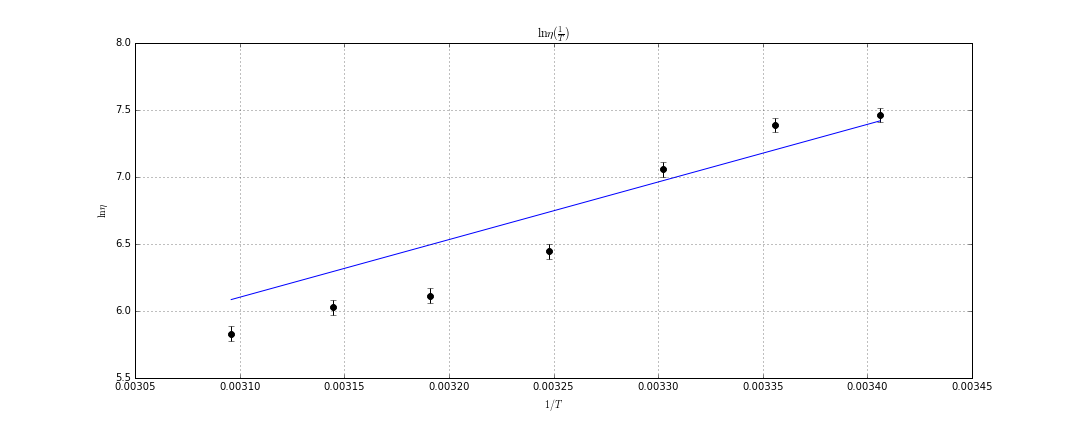
\includegraphics[width=400px, height=180px ]{g1.png} 
                \\ Рис. 1: Воздух
            \end{center}

            Коэффициент наклона прямой по методу наименьших квадратов:  
                \indent $k \approx 211.7$, \quad $\sigma_k \approx 0.5$. \\
            Также учтем ошибку измерения $\sigma_{m} = 5$ \\
            Получим: 
                \indent $v_\text{зв} = 2L k \approx 337 \left[\frac{\text{м}}{c}\right]$, \quad 
             $\sigma_{v_\text{зв}} = 2L \sqrt{\sigma_{k}^2 + \sigma_{m}^2} \approx 8$.
            По формуле (23) найдем $\gamma = C_p/C_v$ :
            \begin{equation}
                \gamma_{\text{воздуха}} = \frac{\mu}{RT}v_\text{зв}^2 \approx 1.34  
            \end{equation}
            
            \begin{equation}
                \sigma_{\gamma} =  \frac{\mu}{R} \sqrt{\left(\frac{2v}{T}\right)^2 (2 \sigma_v)^2 + \left(\frac{v^2}{T^2}\right)^2 \sigma_T^2} \approx 0.07
            \end{equation}

            Табличное значение показателя адиабаты для воздуха при $20^oC$ : $\gamma_{air} \approx 1.4$ 

        \item \underline{$CO_2.$}
        \begin{table}[h]
                    \caption{Резонансные значения частоты для $CO_2$.}
                    \begin{center}
                    \begin{tabular}{|c|c|c|c|c|c|c|c|c|}
                            \hline 
                                $n$ & 1 & 2 & 3 & 4 & 5 & 6 & 7 & 8 \\
                            \hline
                                $f , [Hz]$ &510&672&833&1003&1166&1336&1502&1666\\
                            \hline
                            \end{tabular}
                        \end{center}
            \end{table}
            \begin{center} 
                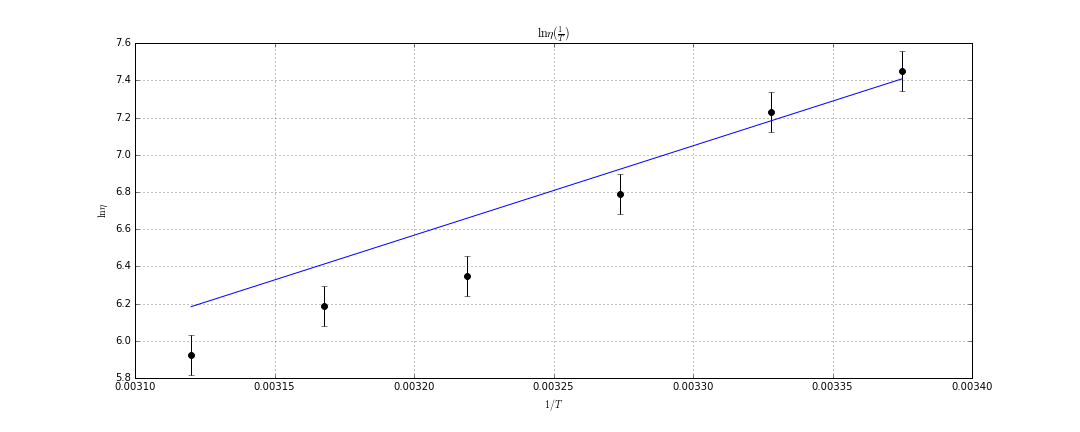
\includegraphics[width=400px, height=180px ]{g2.png} 
                \\ Рис. 2: $CO_2$
            \end{center}
            
            Аналогично: \\
                \indent $k \approx 165.6$, \quad $\sigma_k \approx 0.4$. \\ 
                \indent $v_\text{зв} \approx 263 \left[\frac{\text{м}}{c}\right]$, \quad 
             $\sigma_{v_\text{зв}} = 2L \sqrt{\sigma_{k}^2 + \sigma_{m}^2}  \approx 8$.
            \begin{equation}
                \gamma_{CO_2} \approx 1.24  , \quad \sigma_{\gamma} = 0.08
            \end{equation}
            Табличное значение показателя адиабаты для $CO_2$ при $20^oC$ : $\gamma_{CO_2} \approx 1.3$ 
        \end{enumerate}
        
        \item \underline{Вывод.} \\
        \indent Оптыным путем были получены значения показателей адиабаты $\gamma$ для воздуха и углекислого газа и сравнены с табличными значениями соответствующих величин.
        Полученные результаты, с учетом погрешности, позволяют говорить о применимости модели идеального газа.
    \end{enumerate}

\end{document}